% Options for packages loaded elsewhere
\PassOptionsToPackage{unicode}{hyperref}
\PassOptionsToPackage{hyphens}{url}
\PassOptionsToPackage{dvipsnames,svgnames,x11names}{xcolor}
\documentclass[
  10pt,
  fontset=fandol]{ctexart}
\usepackage{xcolor}
\usepackage[margin=16mm]{geometry}
\usepackage{amsmath,amssymb}
\setcounter{secnumdepth}{-\maxdimen} % remove section numbering
\usepackage{iftex}
\ifPDFTeX
  \usepackage[T1]{fontenc}
  \usepackage[utf8]{inputenc}
  \usepackage{textcomp} % provide euro and other symbols
\else % if luatex or xetex
  \usepackage{unicode-math} % this also loads fontspec
  \defaultfontfeatures{Scale=MatchLowercase}
  \defaultfontfeatures[\rmfamily]{Ligatures=TeX,Scale=1}
\fi
\usepackage{lmodern}
\ifPDFTeX\else
  % xetex/luatex font selection
\fi
% Use upquote if available, for straight quotes in verbatim environments
\IfFileExists{upquote.sty}{\usepackage{upquote}}{}
\IfFileExists{microtype.sty}{% use microtype if available
  \usepackage[]{microtype}
  \UseMicrotypeSet[protrusion]{basicmath} % disable protrusion for tt fonts
}{}
\makeatletter
\@ifundefined{KOMAClassName}{% if non-KOMA class
  \IfFileExists{parskip.sty}{%
    \usepackage{parskip}
  }{% else
    \setlength{\parindent}{0pt}
    \setlength{\parskip}{6pt plus 2pt minus 1pt}}
}{% if KOMA class
  \KOMAoptions{parskip=half}}
\makeatother
\usepackage{graphicx}
\makeatletter
\newsavebox\pandoc@box
\newcommand*\pandocbounded[1]{% scales image to fit in text height/width
  \sbox\pandoc@box{#1}%
  \Gscale@div\@tempa{\textheight}{\dimexpr\ht\pandoc@box+\dp\pandoc@box\relax}%
  \Gscale@div\@tempb{\linewidth}{\wd\pandoc@box}%
  \ifdim\@tempb\p@<\@tempa\p@\let\@tempa\@tempb\fi% select the smaller of both
  \ifdim\@tempa\p@<\p@\scalebox{\@tempa}{\usebox\pandoc@box}%
  \else\usebox{\pandoc@box}%
  \fi%
}
% Set default figure placement to htbp
\def\fps@figure{htbp}
\makeatother
\setlength{\emergencystretch}{3em} % prevent overfull lines
\providecommand{\tightlist}{%
  \setlength{\itemsep}{0pt}\setlength{\parskip}{0pt}}
\usepackage{amsmath,amssymb,mathtools,needspace}
\xeCJKDeclareCharClass{CJK}{"2032,"0400->"04FF,"2160->"216B,"2460->"2473,"25A0,"25C7,"25CB,"25CF}
\IfFontExistsTF{Arial Unicode MS}{\xeCJKsetup{AutoFallBack=true}\setCJKfallbackfamilyfont{\CJKrmdefault}{Arial Unicode MS}}{}
\setcounter{secnumdepth}{0}
\setlength{\emergencystretch}{2em}
\allowdisplaybreaks
\usepackage{bookmark}
\IfFileExists{xurl.sty}{\usepackage{xurl}}{} % add URL line breaks if available
\urlstyle{same}
\hypersetup{
  pdftitle={数值分析研究的对象与特点},
  colorlinks=true,
  linkcolor={Maroon},
  filecolor={Maroon},
  citecolor={Blue},
  urlcolor={Blue},
  pdfcreator={LaTeX via pandoc}}

\title{数值分析研究的对象与特点}
\author{}
\date{}

\begin{document}
\maketitle

\subsubsection{1.1 数值分析研究的对象与特点}\label{ux6570ux503cux5206ux6790ux7814ux7a76ux7684ux5bf9ux8c61ux4e0eux7279ux70b9}

数值分析是研究各种数学问题求解的数值计算方法. 在电子计算机成为数值计算的主要工具以后, 人们迫切要求研究适合于计算机使用的数值计算方法. 为了更具体地说明数值分析的研究对象, 我们来考察用计算机解决科学计算问题时所经历的过程（见图1.1）.

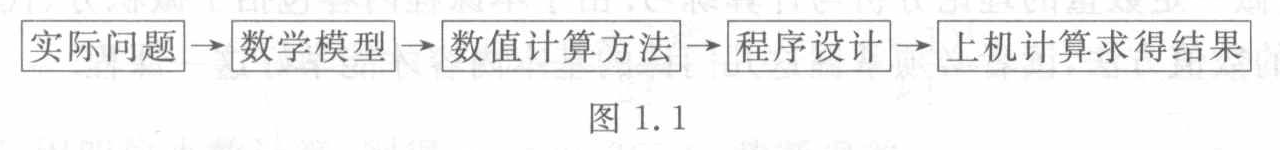
\includegraphics[width=0.85\linewidth,height=\textheight,keepaspectratio,alt={图1.1（原图裁切）}]{../assets/ch01/fig-1-1.png}

图1.1。图中各矩形框依次以向右箭头相连：实际问题 → 数学模型 → 数值计算方法 → 程序设计 → 上机计算求得结果。

由实际问题的提出到上机计算求得结果, 整个过程都可看作应用数学的研究对象. 如果细分的话, 针对实际问题应用有关科学知识和数学理论建立数学模型这一过程, 通常作为应用数学的研究对象, 而根据数学模型提出求解的数值计算方法直到编出程序上机算出结果这一过程, 则是计算数学的研究对象, 也是数值分析的研究对象. 因此, 数值分析就是研究用计算机解决数学问题的数值方法及其理论, 它的内容包括函数的数值逼近、数值微分与数值积分、非线性方程数值解、数值线性代数、微分方程数值解等, 它们都是以数学问题为研究对象的. 因此, 数值分析是数学的一个分支, 只是它不像纯数学那样只研究数学本身的理论, 而是把理论与计算紧密结合起来, 着重研究数学问题的数值方法及其理论.

数值分析也称为计算方法, 但不应片面地将它理解为各种数值方法的简单罗列和堆积. 同数学分析一样, 它内容丰富, 研究方法深刻, 有自身理论体系的课程, 既有纯数学的高度抽象性与严密科学性的特点, 又有应用的广泛性与实际试验的高度技术性的特点, 是一门与计算机应用密切结合的、实用性很强的数学课程. 它与纯数学课程不同, 例如, 在考虑线性方程组数值解时, ``线性代数''中只介绍解存在的唯一性及有关理论和精确解法, 运用这些理论和方法, 无法在计算机上求解上百个未知数的方程组, 更不用说求解十几万个未知数的方程组了. 求解这类问题还应根据方程特点, 研究适合计算机使用的、满足精度要求的、计算省时间的有效算法及其相关的理

\begin{quote}
校注（agent 补充）：本页末尾``理''字与下一页开头``论''字相接。
\end{quote}

\href{../../source-images/pdf-015.jpeg}{查看原页}

论;在实现这些算法时往往还要根据计算机容量、字长、速度等指标,研究具体求解步骤和程序设计技巧;有的方法在理论上虽不够严格,但通过实际计算、对比分析等手段,只要能证明它们是行之有效的方法,也应采用.这些就是数值分析具有的特点,概括起来有四点.

第一,面向计算机,要根据计算机特点提供实际可行的有效算法,即算法只能包括加、减、乘、除运算和逻辑运算,它们都是计算机能直接处理的.

第二,有可靠的理论分析,能任意逼近并达到精度要求,对近似算法要保证收敛性和数值稳定性,还要对误差进行分析.这些都要建立在相应数学理论的基础上.

第三,有好的计算复杂性.时间复杂性好是指节省时间,空间复杂性好是指节省存储量,这也是建立算法要研究的问题,它关系到算法能否在计算机上实现.

第四,有数值实验.任何一个算法,除了从理论上要满足上述三点外,还要通过数值实验证明它是行之有效的.

根据``数值分析''的特点,学习时首先要注意掌握方法的基本原理和思想,要注意方法处理的技巧及其与计算机的结合,要重视误差分析、收敛性及稳定性的基本理论;其次,要通过例子,学习使用各种数值方法解决实际计算问题;最后,为了掌握本课程的内容,还应做一定数量的理论分析与计算练习.由于本课程内容包括了微积分、代数、常微分方程的数值方法,读者必须掌握这几门课的基本内容才能学好这一课程.

\end{document}
